% Chapter Template

\chapter{Experiments evaluation} % Main chapter title

\label{Chapter5} % Change X to a consecutive number; for referencing this chapter elsewhere, use \ref{ChapterX}
In this section we present the results of our experiments in detail. In the first two sections we compare the estimated positions of the three tested algorithms at the given checkpoints. Firstly the results of experiments with wide spread anchors are indicated, secondly the results with nearer anchor positions are shown. In a third section we justify the differences between these two scenarios and comment the accuracy of the results. In the last section we conclude our work and propose next improvement steps for our algorithm. 

%----------------------------------------------------------------------------------------
%	SECTION 1
%----------------------------------------------------------------------------------------

\section{Indoor positioning results with low density of anchor nodes}
In the following the results of our algorithms with a wide distance between anchor nodes are shown. Within this setup we tested trajectory 1 to 4. Each trajectory was tested five times, the results are shown as arithmetic means of these five probes. The anchor node positions for these four tested trajectories are indicated in figure \ref{fig:anchor_position}.

In the first trajectory, the arithmetic mean (hereafter often called average) distance error over all checkpoints was 1.53 meter for $PF_{full}$, 1.47 meter for $PF_{UWBonly}$ and 1.69 meter for Sequiturs commercial system. Looking at figure \ref{fig:trajectory1and2_results}, we see that the errors are often smaller than 1.5 meter, however, there are some checkpoints with very low accuracy. This is also emphasized by comparing the arithmetic mean error to the median error of 1.22m for $PF_{full}$, 0.68m for $PF_{UWBonly}$ and 1.14m for Sequitur, which are significantly lower than the arithmetic means.

The measurements for trajectory two were almost identical, except for $PF_{UWBonly}$, which had no outliers during trajectory 2. The arithmetic mean error for $PF_{full}$ was 2.36m, for $PF_{UWBonly}$ it was 0.55m and for Sequitur 2.26m. Except for $PF_{UWBonly}$, the median errors were again a lot more accurate with 1.07m for $PF_{full}$, 0.49m for $PF_{UWBonly}$ and 1.73m for Sequitur.

\begin{figure}[th]
\centering
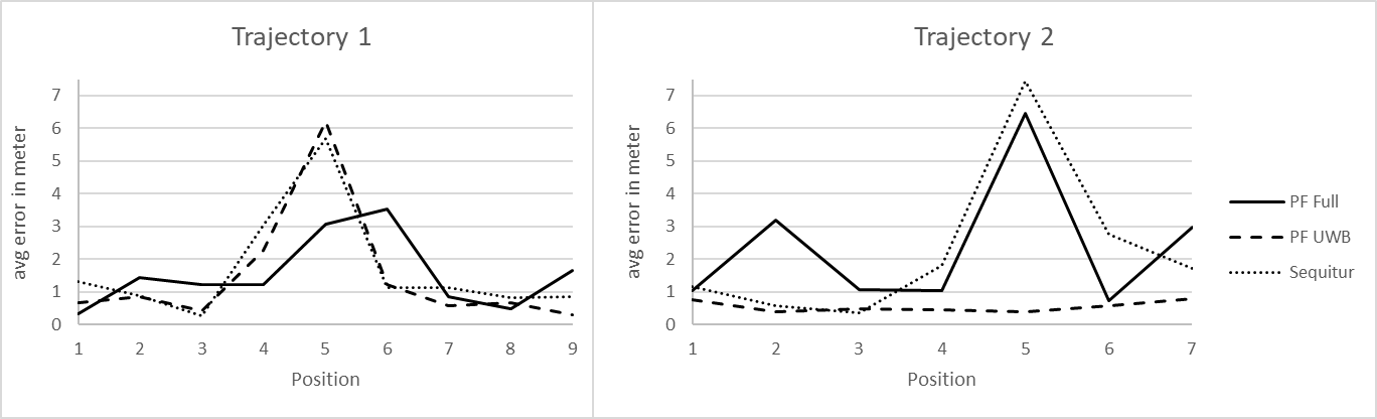
\includegraphics[width=1.0\textwidth]{Figures/trajectory1_2_results}
\decoRule
\caption[Positioning results trajectory 1 and 2]{Graphs of measured distance errors at each checkpoint in trajectory 1, respectively trajectory 2.}
\label{fig:trajectory1and2_results}
\end{figure}

The results for trajectory 3 and 4 were rather similar, however, the peaks observed in figure \ref{fig:trajectory3and4_results} were not as extreme as for the first two trajectories. As above, the average errors in the third trajectory of 1.18m for $PF_{full}$, 0.80m for $PF_{UWBonly}$ and 1.87m for Sequitur were also mentionable higher than the medians of 0.92m, 0.76m and 1.60m.

In the last of these four trajectories no big outliers were stated. Nonetheless the average errors of 1.72m, 1.51m and 1.52m, as well as the median errors 1.26m, 0.68m and 1.24m for $PF_{full}$, $PF_{UWBonly}$ and Sequitur, were still not as accurate as intended.

\begin{figure}[th]
\centering
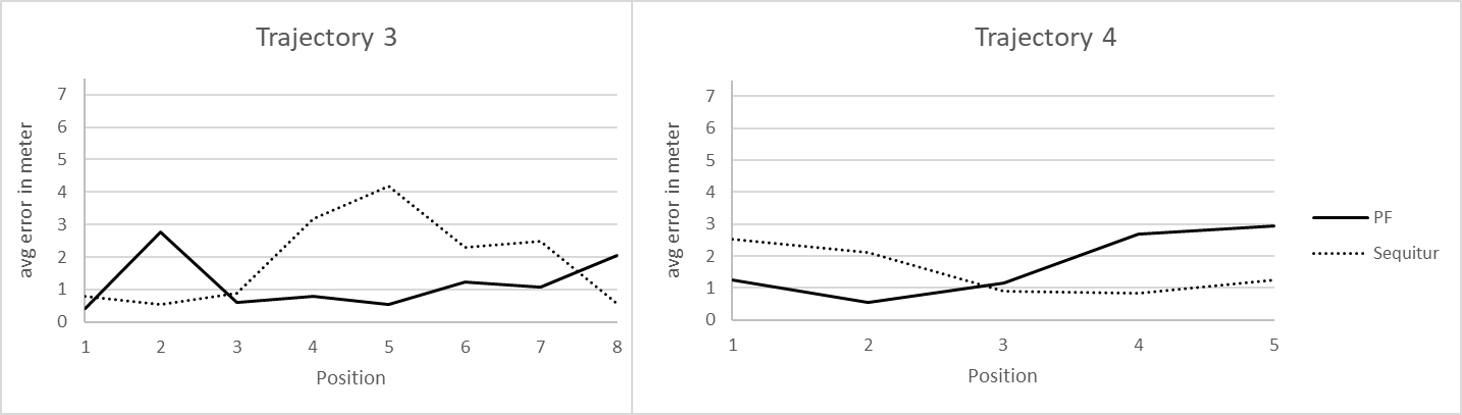
\includegraphics[width=1.0\textwidth]{Figures/trajectory3_4_results}
\decoRule
\caption[Positioning results trajectory 3 and 4]{Graphs of measured distance errors at each checkpoint in trajectory 3, respectively trajectory 4.}
\label{fig:trajectory3and4_results}
\end{figure}

Having a closer look at table \ref{tab:arithmetic_errors}, we see that surprisingly the version of the particle filter only using UWB was the best on every of the trajectories in the low-density anchor node test environment. Moreover, we have seen that there are very big differences between the single checkpoints and even between trajectories. The full variant of the particle filter and the Sequitur system have similar accuracies. For some trajectories one of the algorithms is better, for other trajectories the other one performs better.

\begin{table}
\caption{The arithmetic mean of errors in trajectory 1 to 4 and in total over all measured checkpoints for the three algorithms.}
\label{tab:arithmetic_errors}
\centering
\begin{tabular}{l l l l}
\toprule
\textbf{Trajectory} & \textbf{PF Full} & \textbf{PF UWB} & \textbf{Sequitur}\\
\midrule
\textbf{T1} & 1.54 & 1.47 & 1.69\\
\textbf{T2} & 2.36 & 0.55 & 2.26\\
\textbf{T3} & 1.18 & 0.80 & 1.87\\
\textbf{T4} & 1.72 & 1.51 & 1.52\\
\midrule
\textbf{total}  & \textbf{1.61} & \textbf{1.03} & \textbf{1.79}\\
\bottomrule\\
\end{tabular}
\end{table}



%-----------------------------------
%	SUBSECTION 1
%-----------------------------------

\subsection{Raspberry Pi}
A Raspberry Pi is a single-board computer not much bigger than a credit card. Raspberry Pis are mainly designed for educational purposes as an alternative to expensive notebooks or desk computers. Hence the focus lies also on easy-to-use and plug-and-play experiences. Raspberry Pis are useful for versatile types of projects, as they provide common state of the art hardware - like HDMI, USB and wireless LAN - direct on boad and as they are extendable with selected components.



%-----------------------------------
%	SUBSECTION 2
%-----------------------------------
\subsection{SEQUITUR Pi board with InGPS Lite}
On the 40-pin extended GPIO, we connected the SEQUITUR Pi board from UNISET Company. UNISET is a company located in Italy that focuses on research, development and manufacturing of innovative sensors in two major application areas \cite{Uniset}:

\begin{itemize}
\item Access control security systems, enhancing the reliability of intrusion detection
\item Indoor and outdoor tracking. Sequitur is a precise real time locating system (RTLS) for tracking any object in 2D or 3D with centimeter accuracy.
\end{itemize}
Here goes the text.

%----------------------------------------------------------------------------------------
%	SECTION 2
%----------------------------------------------------------------------------------------

\section{Indoor positioning results with high density of anchor nodes}
Here goes the text.

%-----------------------------------
%	SUBSECTION 1
%-----------------------------------
\subsection{Transmission}
Here goes the text.
%-----------------------------------
%	SUBSECTION 2
%-----------------------------------
\subsection{Ranging with TWR}
Here goes the text.

%----------------------------------------------------------------------------------------
%	SECTION 3
%----------------------------------------------------------------------------------------

\section{Comment}
Here goes the text.
\begin{itemize}
\item Spread the particles and validate new positions with floormap constraints
\item Evaluate UWB ranges, IMU measures and zone indication to assign likelihood
\item Calculate weight function and systematically resample (and reposition) particles with low weights
\item Sum up weighted positions
\end{itemize}

%-----------------------------------
%	SUBSECTION 1
%-----------------------------------
\subsection{Inputs}
Here goes the text.



%-----------------------------------
%	SUBSECTION 2
%-----------------------------------
\subsection{Likelihood and weighting}
Here goes the text.


%-----------------------------------
%	SUBSECTION 3
%-----------------------------------
\subsection{Ranging with TWR}
Here goes the text.



%----------------------------------------------------------------------------------------
%	SECTION 4
%----------------------------------------------------------------------------------------

\section{Conclusion and further work}
Here goes the text.
\begin{itemize}
\item Spread the particles and validate new positions with floormap constraints
\item Evaluate UWB ranges, IMU measures and zone indication to assign likelihood
\item Calculate weight function and systematically resample (and reposition) particles with low weights
\item Sum up weighted positions
\end{itemize}
